%-------------------------------------------------------------
% Fichier: specifications.tex    Auteur(s): Simon DÉSAULNIERS
% Date: 2013-04-24
%-------------------------------------------------------------
% Document de spécification du code pour le projet de
% session du cours INF1009 à l'Université du Québec à
% Trois-Rivières
%-------------------------------------------------------------
\documentclass[11pt,french]{article}

\usepackage[frenchb]{babel}
\usepackage[utf8]{inputenc}
\usepackage[T1]{fontenc}

\usepackage{graphicx}

\usepackage{hyperref}
\hypersetup{hidelinks}

% Style des pages
\usepackage{fancyhdr}
\pagestyle{fancy}
\lhead{Travail de Session}

% Caractères mathématiques
\usepackage{amssymb}

\usepackage{color}

\usepackage[final]{pdfpages}

% Affichage de code source
\usepackage{listings}
\definecolor{dkgreen}{rgb}{0,0.6,0}
\definecolor{dkblue}{rgb}{0,0,0.8}
\definecolor{gray}{rgb}{0.5,0.5,0.5}
\definecolor{mauve}{rgb}{0.58,0,0.82}

\usepackage{courier}

\lstset{ %
backgroundcolor=\color{white},   % choose the background color; you must add \usepackage{color} or \usepackage{xcolor}
basicstyle=\footnotesize,        % the size of the fonts that are used for the code
breakatwhitespace=false,         % sets if automatic breaks should only happen at whitespace
breaklines=true,                 % sets automatic line breaking
captionpos=b,                    % sets the caption-position to bottom
commentstyle=\color{dkblue},    % comment style
deletekeywords={...},            % if you want to delete keywords from the given language
escapeinside={\%*}{*)},          % if you want to add LaTeX within your code
extendedchars=true,              % lets you use non-ASCII characters; for 8-bits encodings only, does not work with UTF-8
frame=single,                    % adds a frame around the code
keywordstyle=\color{dkgreen},       % keyword style
morekeywords={*,...},            % if you want to add more keywords to the set
numbers=left,                    % where to put the line-numbers; possible values are (none, left, right)
numbersep=5pt,                   % how far the line-numbers are from the code
numberstyle=\tiny\color{gray}, % the style that is used for the line-numbers
rulecolor=\color{black},         % if not set, the frame-color may be changed on line-breaks within not-black text (e.g. comments (green here))
showspaces=false,                % show spaces everywhere adding particular underscores; it overrides 'showstringspaces'
showstringspaces=false,          % underline spaces within strings only
showtabs=false,                  % show tabs within strings adding particular underscores
stepnumber=2,                    % the step between two line-numbers. If it's 1, each line will be numbered
stringstyle=\color{red},     % string literal style
tabsize=2,                       % sets default tabsize to 2 spaces
xleftmargin=\parindent,
title=\lstname                   % show the filename of files included with \lstinputlisting; also try caption instead of title
}


\newcommand{\HRule}{\rule{\linewidth}{0.5mm}}

\begin{document}
    % PAGE TITRE
    \begin{titlepage}
        \begin{center}
    
            
\includegraphics[height=3cm]{./aux/network.png}
            \\[3cm]
            
            \textsc{\LARGE Réseaux d'ordinateurs I}
            \\[0.2cm]
            \textsc{\Large INF1009}
            \\[2cm]
            \HRule \\[0.5cm]
            {\huge \bfseries Travail de Session}
            \HRule \\[2cm]
            Par\\
            Simon Désaulniers

            \vfill
            2013-04-24\\
            Université du Québec à Trois-Rivières
            \thispagestyle{empty}
        \end{center}
    \end{titlepage}
    \newpage

    % TABLE DES MATIÈRES
    \pagenumbering{roman}
    \setcounter{page}{1}
    \tableofcontents
    \newpage

    % CORPS DU RAPPORT
    \pagenumbering{arabic}
    \setcounter{page}{1}
    
    \section*{Introduction} % (fold)
    \label{sec:intro}
        Le présent document est destiné à la meilleure compréhension de la conception
        du programme réalisé pour le cours \emph{INF1009}. Les différents fichiers sources
        \footnote{Le code source est disponible à l'adresse {\color{blue}\href{https://github.com/sim590/inf1009-tp}{https://github.com/sim590/inf1009-tp}}}
        seront détaillés afin d'expliquer les choix qui ont été faits lors de l'écriture
        de ceux-ci.\\

        Le projet est réalisé suivant les spécifications de l'éconcé en annexe et donc demeure
        fonctionnel dans un environnement utilisant la norme \emph{POSIX}\footnote{Comme les
        différentes distributions \emph{GNU/Linux} (Debian, Ubuntu, Linux Mint, etc.)}.
    % section intro (end)
    
    \lstset{language=make}
    \section{Makefile} % (fold)
    \label{sec:makefile}
        Le fichier nommé \emph{Makefile} permet de compiler\footnote{La compilation utilise le programme
        gcc (GNU C/C++ Compiler).} les différents fichiers sources
        à l'aide d'une seule commande entrée au terminal \texttt{make all}. Lorsque cette commande
        est envoyée au terminal et que répertoire de travail est le même que le fichier \emph{Makefile},
        la règle \texttt{all} est appellée.
        \lstinputlisting[firstline=13,lastline=13]{../Makefile}
        Celle-ci appelle ses dépendences et ainsi compile tous les 
        fichiers sources.
        \lstinputlisting[firstline=14,lastline=42]{../Makefile}

        Une fois les fichiers compilés et liés dans 3 objets binaires
        {\bf inf1009-tp}, {\bf transport-entity} et {\bf network-entity},
        il est possible de lancer le programme en appellant\footnote{Il est recommandé de
        démarrer le programme à l'aide d'un terminal afin d'avoir différentes informations sur
        la sortie standard.} le programme \emph{inf1009-tp}.
        Bien-sûr, le programme nécessite le fichier \emph{S\_LEC} afin d'obtenir des informations et
        ainsi produire les résultats attendus dans les autres fichiers \emph{S\_ECR}, \emph{L\_LEC}
        et \emph{L\_ECR}.\\

        Le script permet aussi de nettoyer le répertoire des fichiers sources et des fichiers binaires
        en utilisant respectivement la commande \texttt{make clean} et \texttt{make cleanbin}.
        \lstinputlisting[firstline=44,lastline=48]{../Makefile}
    % section makefile (end)
    
    \lstset{language=c}
    
    \section{inf1009-tp} % (fold)
    \label{sec:inf1009-tp}
        Ce programme est compilé à l'aide du fichier \emph{main.c}. C'est le programme qui appelle
        les deux processus ET\footnote{Entité Transport} et ER\footnote{Entité Réseau}. Il nécessite
        que les deux programmes soient dans le même répertoire
        
        \subsection{Fichiers d'en-têtes} % (fold)
        \label{sub:fich-entete}
            
            \subsubsection{main.h} % (fold)
            \label{ssub:main.h}
                Le fichier \emph{main.h} contient les appels aux librairies nécessaires ainsi que la déclaration
                d'une fonction à laquelle on fait appel dans le fichier \emph{main.c}.
                \lstinputlisting{../src/main.h}
            % subsubsection main.h (end)
        % subsection fich-entete (end)
        \subsection{Fichiers d'implémentation} % (fold)
        \label{sub:fich-compiles-inf1009-tp}
        
        \subsubsection{main.c} % (fold)
        \label{ssub:main.c}
            Ce fichier consiste en la routine du programme {\bf inf1009-tp}. En premier lieu, il fait l'ouverture de tuyaux de communication
            afin que les deux processus ET et ER puissent échanger.
            \lstinputlisting[firstline=15,lastline=26]{../src/main.c}

            Par la suite, à l'aide de la fonction \texttt{fork()}, il duplique le processus parent et créé un premier processus enfant.
            \lstinputlisting[firstline=30,lastline=30]{../src/main.c}

            L'image du processus enfant est alors écrasé par celle du programme {\bf transport-entity} au moyen de la fonction de la famille
            \texttt{exec}.
            \lstinputlisting[firstline=37,lastline=52]{../src/main.c}
            
            Le parent répète alors le même processus pour créer un deuxième processus enfant, c-à-d le processus exécutant le programme
            {\bf network-entity}.
            \lstinputlisting[firstline=55,lastline=76]{../src/main.c}

            Ceci étant fait, le processus {\bf inf1009-tp} peut maintenant se terminer et laisser les deux processus ET et ER effectuer le reste.
        % subsubsection main.c (end)
        % subsection fich-compiles (end)
    % section inf1009-tp (end)

    \section{transport-entity} % (fold)
    \label{sec:transport-entity}
        Ce programme est compilé à l'aide des fichiers \emph{transport.c} et \emph{transNnet.c}. Lorsque ce processus est en marche, il fait la lecture
        du fichier \emph{S\_LEC} afin d'obtenir la transaction de la couche session\footnote{Cette couche n'est pas implémentée dans le projet, mais est
        simulée au moyen de deux fichiers \emph{S\_LEC} et \emph{S\_ECR}} pour la transmettre à la couche réseau. De plus,
	il écrit les messages qu'il reçoit de la couche réseau dans le fichier \emph{S\_ECR}.
	
	\subsection{Fichiers d'en-têtes}
	\label{sub:fich-entetes-transport-entity}
		\subsubsection{transNnet.h}
		\label{ssub:transNnet.h}
			Le fichier \emph{transNnet.h} contient toute déclaration de librairies, variables, structures et fonctions utiles
			autant dans le processus \emph{ET} que \emph{ER}.\\

			Afin de permettre aux processus d'attendre un temps maximal après l'autre à l'écoute d'un tuyau,
			on définit le nombre suivant:
			\lstinputlisting[firstline=14,lastline=14]{../src/transNnet.h}

            \vspace{0.5cm}

            On retrouve les librairies suivantes:
            \lstinputlisting[firstline=17,lastline=21]{../src/transNnet.h}

            \vspace{0.5cm}

			On retrouve l'énumération et les structures suivantes:
			
            \lstinputlisting[firstline=28,lastline=40]{../src/transNnet.h}
			Cette énumération permet de passer facilement les primitives de communication entre les deux couches implémentées.
			
            \lstinputlisting[firstline=46,lastline=51]{../src/transNnet.h}
            C'est la forme selon laquelle on construit une requête lors de la phase de connexion autant du côté de \emph{ET} que de \emph{ER}. 
            La structure est composée d'une primitive, un numéro de connexion, une adresse source et une adresse de destination.

            \lstinputlisting[firstline=53,lastline=57]{../src/transNnet.h}
            C'est la forme selon laquelle on construit une requête lors de la phase de transmission de données. La structure est composée d'une primitive,
            un numéro de connexion et une transaction\footnote{La transaction est prise dans le fichier \emph{S\_LEC} avec le numéro correspondant}.

            \lstinputlisting[firstline=59,lastline=62]{../src/transNnet.h}
            C'est la forme selon laquelle on construit une requête lors de la phase de libération de connexion. On fournit une primitive ainsi qu'un 
            numéro de connexion.

            \lstinputlisting[firstline=68,lastline=73]{../src/transNnet.h}
            On utilise l'union afin de rendre transparente la construction d'un paquet. Autrement dit, le programme créé toujours des structures spéciales 
            du type \texttt{PRIM\_PACKET} et ainsi un seul des champ de cette structure est initialisée. La primitive sert de clée afin de savoir de
            quelle\footnote{Dans une union, tous les champs partagent le même espace mémoire.} structure on parle à tout moment.

            \lstinputlisting[firstline=79,lastline=83]{../src/transNnet.h}
            Cette structure permet de créer une liste chaînée de connexions et ainsi garder le suivi des connexions en cours du côté de l'\emph{ET}. 
            Chaque noeud est composé d'un numéro de connexion, un état de connexion et un pointeur vers la connexion suivante.

            \lstinputlisting[firstline=89,lastline=95]{../src/transNnet.h}
            Identique à la structure précédente mis-à-part du point qu'elle est utilisée du côté de l'\emph{ER} et qu'elle possède une adresse source et
            de destination pour chaque connexion.

            \lstinputlisting[firstline=97,lastline=100]{../src/transNnet.h}
            Permet une manipulation transparente des structures de connexion (même principe que l'union précédente).\\

            De plus, on retrouve la déclaration des différentes fonctions définies dans le fichier \emph{transNnet.c}.
            \lstinputlisting[firstline=106,lastline=106]{../src/transNnet.h}
            Cette fonction permet d'écouter sur le tuyau demandé la réponse de l'interlocuteur. On passe en paramètre un pointeur vers un paquet \texttt{PRIM\_PACKET}
            dans lequel on souhaite stocker les informations tirées du tuyau identifié par un entier.
            \lstinputlisting[firstline=107,lastline=107]{../src/transNnet.h}
            À l'aide de cette fonction, l'entité transport ou réseau d'écrire sur le tuyau spécifié par un entier. On passe en paramètre un pointeur vers un paquet \texttt{PRIM\_PACKET}
            qu'on souhaite transmettre à l'interlocuteur.
            \lstinputlisting[firstline=108,lastline=108]{../src/transNnet.h}
            Détruit la liste chaînée de connexions afin de libérer les ressources utilisés à la fin de l'exécution du processus en question.
            \lstinputlisting[firstline=109,lastline=109]{../src/transNnet.h}
            Trouve une connexion dans la liste chaînée. Si celle-ci s'y trouve, la fonction renvoie un pointeur vers elle, autrement elle renvoie la valeur constante \texttt{NULL}.
            \lstinputlisting[firstline=110,lastline=110]{../src/transNnet.h}
            Ajoute une connexion à la liste chaînée. On passe en paramètre le numéro de connexion. Si l'entité réseau utilise cette fonction, elle passera une adresse source et une 
            adresse destination, sinon si c'est l'entité transport, celle-ci ne fait que passer la valeur \texttt{NULL} aux autres paramètres.
            \lstinputlisting[firstline=111,lastline=111]{../src/transNnet.h}
            Retire une connexion de la liste chaînée. On passe le numéro de connexion en paramètre.
            \lstinputlisting[firstline=112,lastline=112]{../src/transNnet.h}
            Écriture d'informations relatives à la communication entre ET et ER sur la sortie standard.
		% subsubsection transNnet.h
        \subsubsection{transport.h} % (fold)
        \label{ssub:transport.h}
			Le fichier \emph{transport.h} est le fichier d'en-tête principal du fichier d'implémentation \emph{transport.c}. Il contient toute déclaration de librairies, 
            variables, structures et fonctions utile autant dans le processus \emph{ET} que \emph{ER}.\\
            
            \vspace{0.5cm}
            
            On définit quelques variables:
            \lstinputlisting[firstline=11,lastline=12]{../src/transport.h}
            C'est le nom de fichiers statiques et importants au déroulement du processus.

            \lstinputlisting[firstline=13,lastline=13]{../src/transport.h}
            Variable permettant d'identifier le processus lors de l'utilisation de fonctions déclarées de façon communes à \emph{ET} et \emph{ER}.
            
            \vspace{0.5cm}

            On inclue des fichiers d'en-tête:
            \lstinputlisting[firstline=15,lastline=15]{../src/transport.h}

            \vspace{0.5cm}

            On déclare les fonctions suivantes:
            \lstinputlisting[firstline=19,lastline=19]{../src/transport.h}
            Cette fonction permet d'extraire le message à envoyer de la ligne recueilli du fichier \emph{S\_LEC}.
            \lstinputlisting[firstline=20,lastline=20]{../src/transport.h}
            Celle-ci écrit les résultats dans le fichiers \emph{S\_ECR}.
        % subsubsection transport.h (end)
	% subsection fich-entetes-transport-entity (end)
    \subsection{Fichiers d'implémentation} % (fold)
    \label{sub:fich-implementation-trans-entity}
        \subsubsection{transNnet.c} % (fold)
        \label{ssub:transNnet.c}
            Ce fichier décrit une interface commune entre l'entité transport et l'entité réseau. Afin de communiquer, chacune des entités utilisera les fonctions déclarées dans le fichier
            \emph{transNnet.h} et définies dans le fichier \emph{transNnet.c}.
        % subsubsection transNnet.c (end)
        \subsubsection{transport.c} % (fold)
        \label{ssub:transport.c}
            Ce fichier décrit la routine du processus \emph{ET}. De façon rapide, il est suffisant d'observer le pseudo-code de l'algorithme suivant:
\begin{lstlisting}
TANT QUE FICHIER_NON_VIDE
    LIRE S_LEC
    
    REGARDER_TABLE_DE_CONNEXIONS
    
    SI CONNEXION_EXISTE_PAS
        ENVOYER_CONNECTION_REQ
        ECOUTER_REPONSE
        
        SI REPONSE_POSITIVE
            CHANGER_ETAT_CONNEXION_TABLE_CONNEXION
            ENVOYER_DATA_REQ
        SINON
            SUPPRIMER_CONNEXION
        FIN SI
    SINON
        ENVOYER_DATA_REQ
    FIN SI
FIN TANT QUE

POUR TOUTES LES CONNEXIONS
    SUPPRIMMER_CONNEXION
\end{lstlisting}
            
        % subsubsection transport.c (end)
    % subsection fich-implementation-trans-entity (end)
    % section transport-entity (end)

    \section{network-entity} % (fold)
    \label{sec:network-entity}
        Ce programme est compilé à l'aide des fichiers \emph{network.c} et \emph{transNnet.c}. Le processus étant lancé, il écoute les requêtes de l'entité transport afin de les soumettre
        à plusieurs tests. Il vérifie différentes conditions nécessaire à l'acheminement des requêtes de \emph{ET} et simule la réponse d'un système distant en écrivant celle-ci dans la
        couche liaison (simulée par les fichiers \emph{L\_LEC} et \emph{L\_ECR}).

        \subsection{Fichiers d'en-têtes} % (fold)
        \label{sub:Fichiers d'en-têtes}
        
            \subsubsection{network.h} % (fold)
            \label{ssub:network.h}
                Ce fichier consiste en l'en-tête principale du fichier d'implémentation \emph{network.c}. Il contient les différentes déclarations de structures, fonctions, librairies et variables
                utiles au processus \emph{ER}.\\

                On définie les constantes suivantes:
                \lstinputlisting[firstline=13,lastline=14]{../src/network.h}
                Chemin vers les fichiers nécessaire au bon fonctionnement du processus \emph{ER}.
                \lstinputlisting[firstline=16,lastline=16]{../src/network.h}
                Chaîne de caractères constante permettant d'identifier le processus lors de l'utilisation de l'interface définie dans \emph{transNnet.c}.

                \vspace{0.5cm}

                On inclue des fichiers d'en-tête:
                \lstinputlisting[firstline=18,lastline=18]{../src/network.h}

                \vspace{0.5cm}

                On retrouve les émumérations et structures suivantes:
                \lstinputlisting[firstline=26,lastline=30]{../src/network.h}
                Énumération des types de paquets admissibles lors de la phase de connexion.
                \lstinputlisting[firstline=32,lastline=35]{../src/network.h}
                Énumération des raisons fournies dans un paquet lors d'une libération de connexion.
                \lstinputlisting[firstline=41,lastline=48]{../src/network.h}
                Paquet manipulé lors de la phase de connexion. Il est composé d'un type de paquet, un type de paquet de connexion, un numéro de connexion, une adresse source, une adresse destination et
                un champ raison utilisé lors du refus de connexion.
                \lstinputlisting[firstline=70,lastline=75]{../src/network.h}
                Paquet de données utilisé lors de la phase de transmission de données. Il est composé d'un type de paquet, un type, un numéro de connexion ainsi que d'un segment de données.
                \lstinputlisting[firstline=81,lastline=87]{../src/network.h}
                Paquet de libération utilisé lors de la phase de libération de connexion initiée par le destinateur. Il est composé d'un type de paquet, un type, un numéro de connexion, une adresse source et adresse destination.
                \lstinputlisting[firstline=92,lastline=97]{../src/network.h}
                Union permettant une écriture transparente du code. Les structures mentionnées plus haut partagent tous un même espace mémoire à l'intérieure d'une union.
                
                \vspace{0.5cm}

                On déclare les fonctions suivantes:
                \lstinputlisting[firstline=99,lastline=99]{../src/network.h}
                Envoie un paquet de données vers la couche liaison. On passe en paramètre un pointeur vers le paquet préalablement construit et le chemin\footnote{Il est important de se rappeller que le système distant est
                simulé et donc, c'est le processus \emph{ER} qui écrira dans les deux fichiers} vers le fichier dans lequel on souhaite écrire le paquet.
                \lstinputlisting[firstline=100,lastline=100]{../src/network.h}
                Génère la réponse du système distant. On passe en paramètre un pointeur vers le paquet précédemment envoyé à la couche liaison.
            % subsubsection network.h (end)
            \subsubsection{transNnet.h} % (fold)
            \label{ssub:transNnet.h-net}
                Voir section {\color{blue} \ref{ssub:transNnet.h}}
            % subsubsection transNnet.h-net (end)
        % subsection Fichiers d'en-têtes (end)
        \subsection{Fichier d'implémentation} % (fold)
        \label{sub:fich-implementation-network-entity}
            \subsubsection{network.c} % (fold)
            \label{ssub:network.c}
                Ce fichier consiste en la routine de l'entité réseau. Afin de comprendre ce que fait celui-ci, il est suffisant d'observer le pseudo-code suivant:
\begin{lstlisting}
TANT QUE MESSAGE_DANS_TUYAU
    SI N_CONNECT_REQ
        SI ER_ACCEPTE
            SI CONNEXION_NEXISTE_PAS
                AJOUTER_CONNEXION
            FIN SI

            CONSTRUIRE_CONNECTION_PACKET

            ECRIRE_CONNECTION_PACKET(L_ECR)

            GEN_REPONSE_B

            ECRIRE_REPONSE_B(L_LEC)
            SI REPONSE_B_OUI
                REPONDRE_ET_OUI_B
            SINON
                REPONDRE_ET_NON_B
        SINON
            REPONDRE_ET_NON
    SINON SI N_DATA_REQ
        SEGMENTER_MESSAGE
        
        POUR TOUT SEGMENTS
            ECRIRE_DATA_PACKET(L_ECR)
            GEN_REPONSE_B
            
            ECRIRE_REPONSE_B(L_LEC)
            SI AUCUNE_REPONSE OU REPONSE_NEGATIVE
                ECRIRE_DATA_PACKET(L_ECR)
                GEN_REPONSE_B
                
                ECRIRE_REPONSE_B
            FIN SI
        FIN POUR TOUT
    SINON SI N_DISCONNECT_REQ
        ECRIRE_REL_PACKET(L_ECR)
    FIN SI
FIN TANT QUE
\end{lstlisting}
            % subsubsection network.c (end)
            \subsubsection{transNnet.c} % (fold)
            \label{ssub:transNnet.c-net}
                Voir section {\color{blue} \ref{ssub:transNnet.c}}
            % subsubsection transNnet.c-net (end)
        % subsection fich-implementation-network-entity (end)
    % section network-entity (end)
    \newpage
    \section{ANNEXES} % (fold)
    \label{sec:ANNEXES}
        \subsection*{ANNEXE A: Projet de Réseaux} % (fold)
        \label{sub:ANNEXE A: Projet de Réseaux}
        
        % subsection ANNEXE A: Projet de Réseaux (end)
        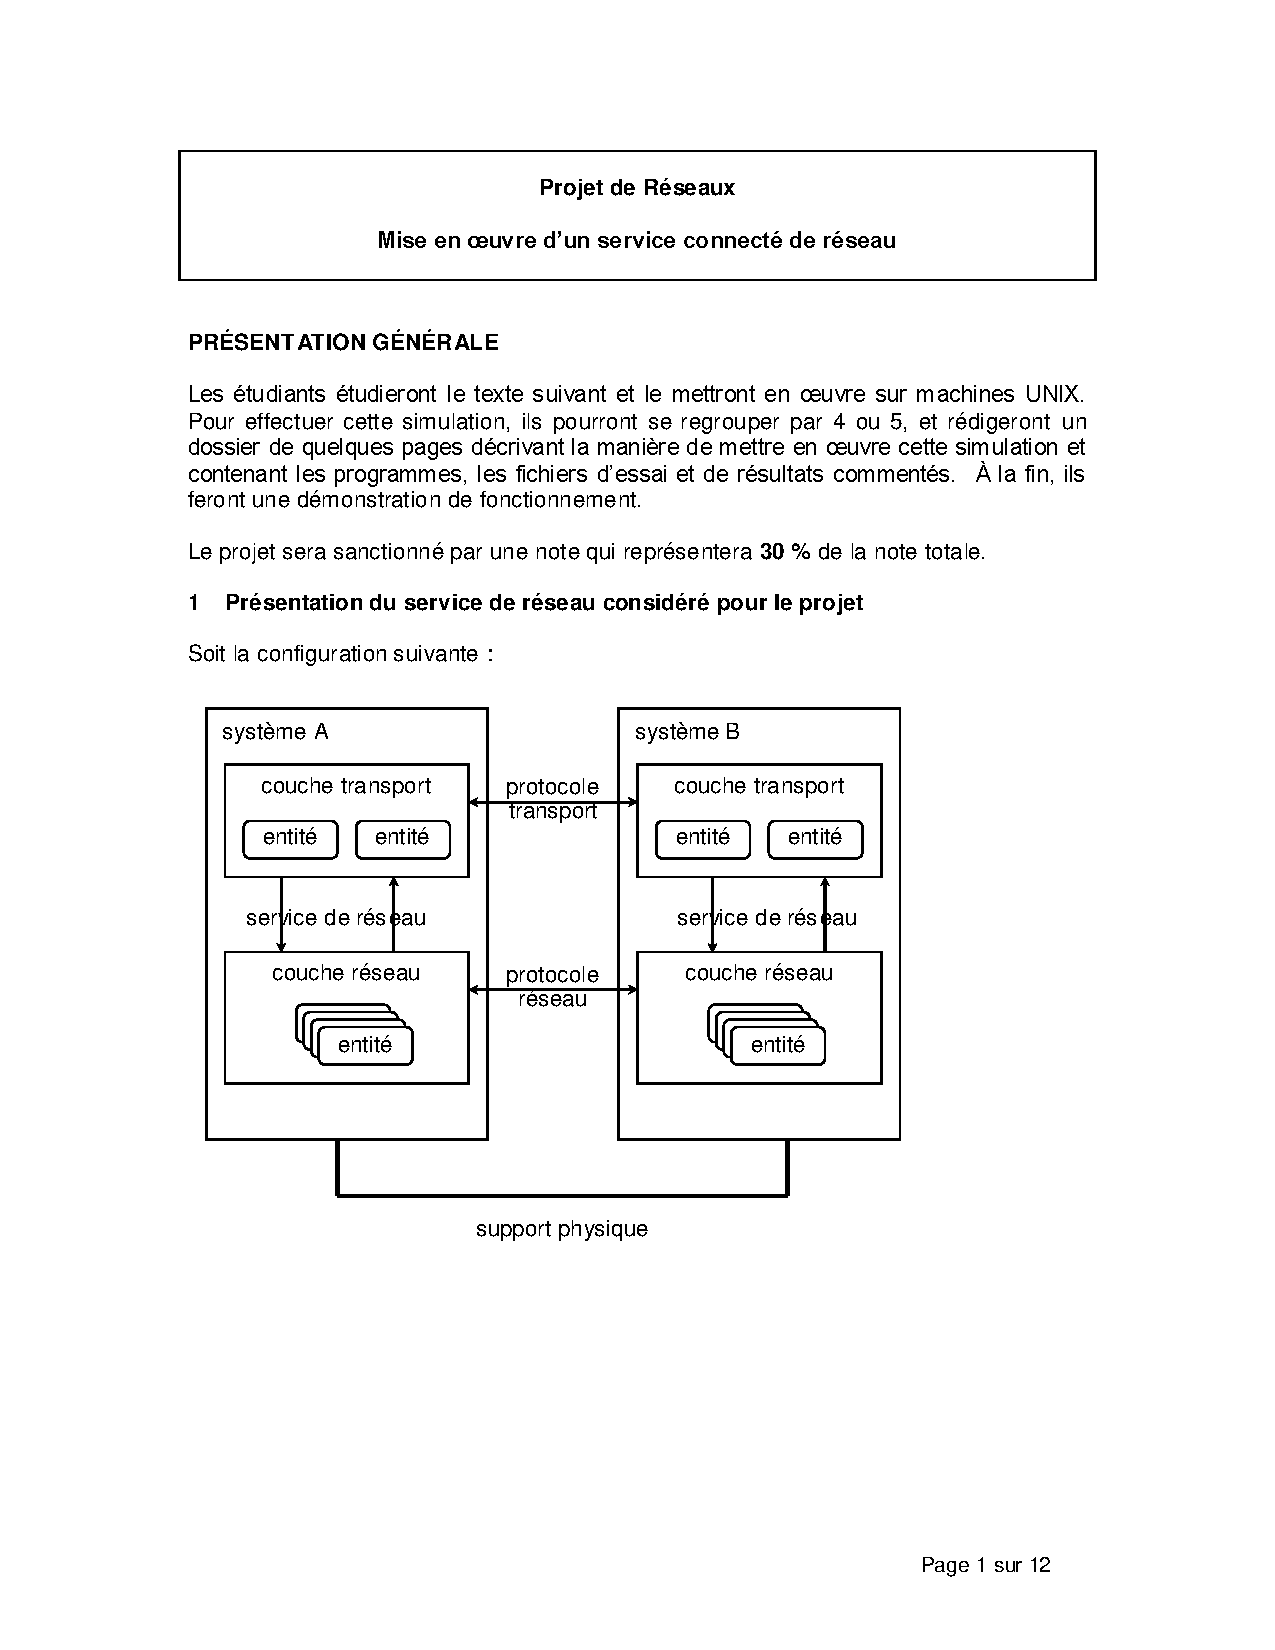
\includepdf[pages=1-12]{./aux/enonce-tp.pdf}
    % section ANNEXES (end)
\end{document}
